%============================================================
%  Capitolo 0 – Introduzione al Deep Learning
%============================================================
\chapter{Introduzione al Deep Learning}
\label{ch:intro}

La veloce crescita odierna del Machine Learning ha portato alla nascita di nuove
tecnologie e campi di applicazione. Il \textbf{Deep Learning} nasce con
l'intento di apprendere rappresentazioni gerarchiche direttamente dai dati,
tramite reti neurali profonde. I campi di applicazione spaziano dalla
diagnostica medica fino ai Large Language Models (LLM) \citep{bishop2024}.

%------------------------------------------------------------
\section{Machine Learning vs Deep Learning}
\label{sec:ml-vs-dl}

Nel \textbf{Machine Learning classico} la pipeline si divide in due fasi
nettamente separate: un'estrazione di feature progettata manualmente
dall'ingegnere, seguita da un classificatore appreso automaticamente dai dati.
Nel \textbf{Deep Learning} entrambe le fasi sono apprese congiuntamente e in
modo gerarchico: i layer bassi catturano edge e texture, quelli intermedi parti
di oggetti, quelli alti concetti semantici \citep{lecun2021}.

\begin{figure}[H]
  \centering
  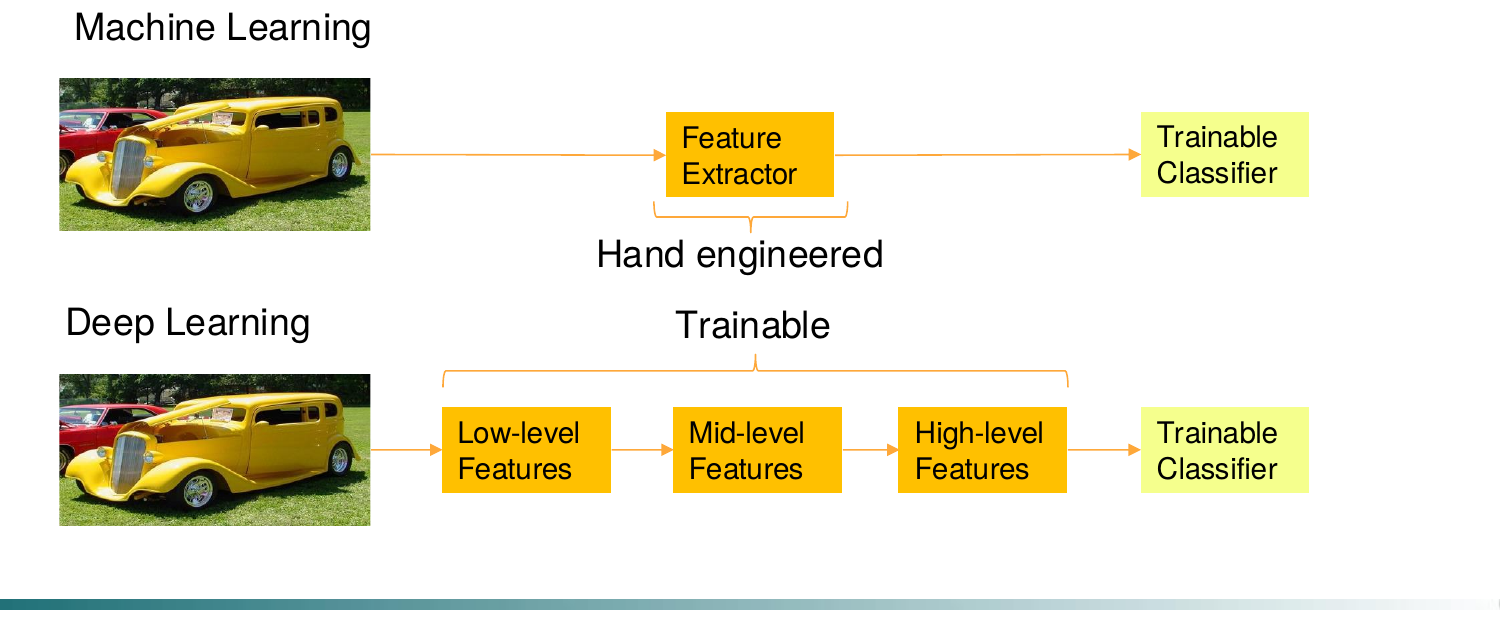
\includegraphics[width=0.88\linewidth]{figures/ml_vs_dl.png}
  \caption{Confronto tra la pipeline di ML classico (feature extractor
           hand-engineered + classificatore) e quella di Deep Learning
           (tutta la catena è trainable end-to-end).}
  \label{fig:ml_vs_dl}
\end{figure}

Il Deep Learning si colloca all'interno della gerarchia
\textit{AI} $\supset$ \textit{Machine Learning} $\supset$
\textit{Representation Learning} $\supset$ \textit{Deep Learning}.
La figura seguente mostra questa gerarchia e il corrispondente spettro
di paradigmi, dal rule-based al deep learning.

\begin{figure}[H]
  \centering
  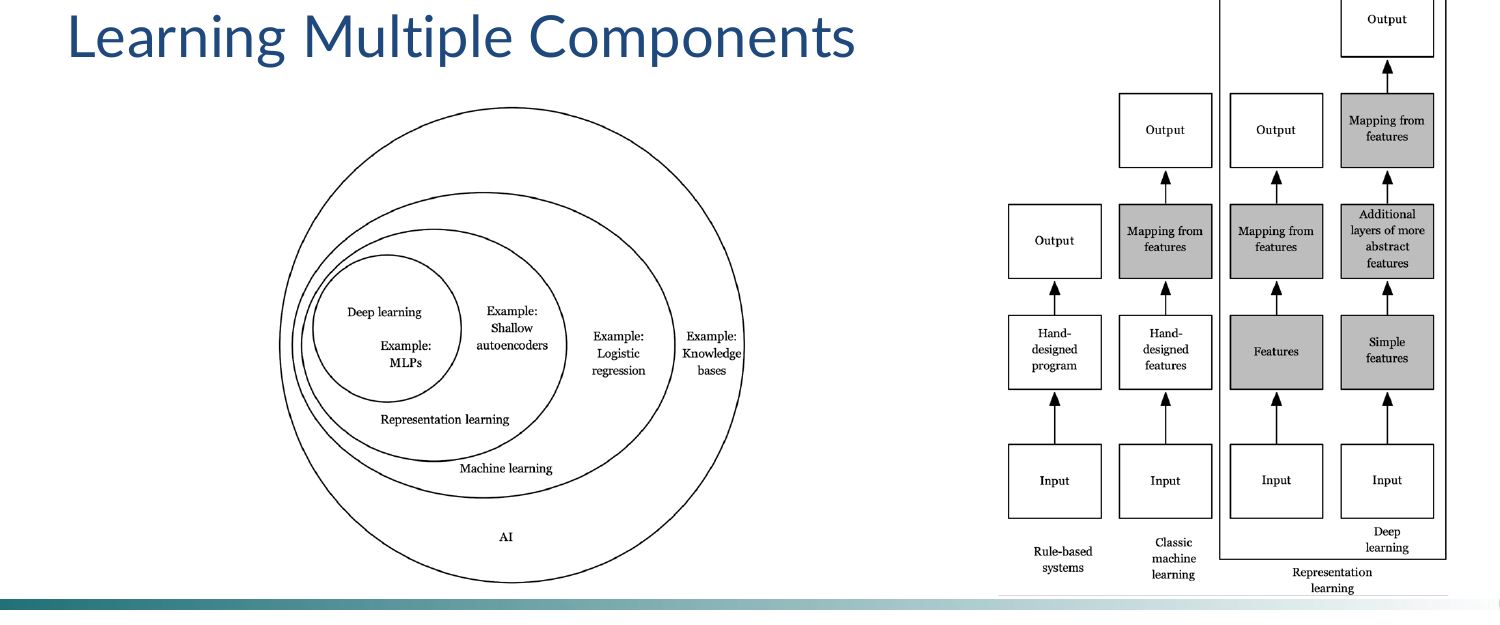
\includegraphics[width=0.92\linewidth]{figures/learning_components.png}
  \caption{Gerarchia AI/ML/Repr.\,Learning/DL (sinistra) e i quattro
           paradigmi principali con il loro grado di automazione (destra).}
  \label{fig:learning_components}
\end{figure}

Un esempio storico di benchmark è il dataset \textbf{MNIST} \citep{lecun1998}:
$70\,000$ immagini $28{\times}28$ pixel di cifre scritte a mano (0--9).
Un MLP semplice raggiunge circa il 98\% di accuratezza; la CNN LeNet-5 arriva
al 99.3\%.

%------------------------------------------------------------
\section{Modello Parametrico e Funzione di Costo}
\label{sec:parameterized-model}

Un \textbf{modello parametrico} è una funzione deterministica della forma
\begin{equation}
  \bar{y} = G(x,\, w)
\end{equation}
dove $x$ è l'ingresso osservato, $w$ il vettore dei parametri addestrabili
e $\bar{y}$ l'uscita predetta. I parametri $w$ sono condivisi tra tutti i
campioni di addestramento, mentre $x$ varia da campione a campione.

\begin{figure}[H]
  \centering
  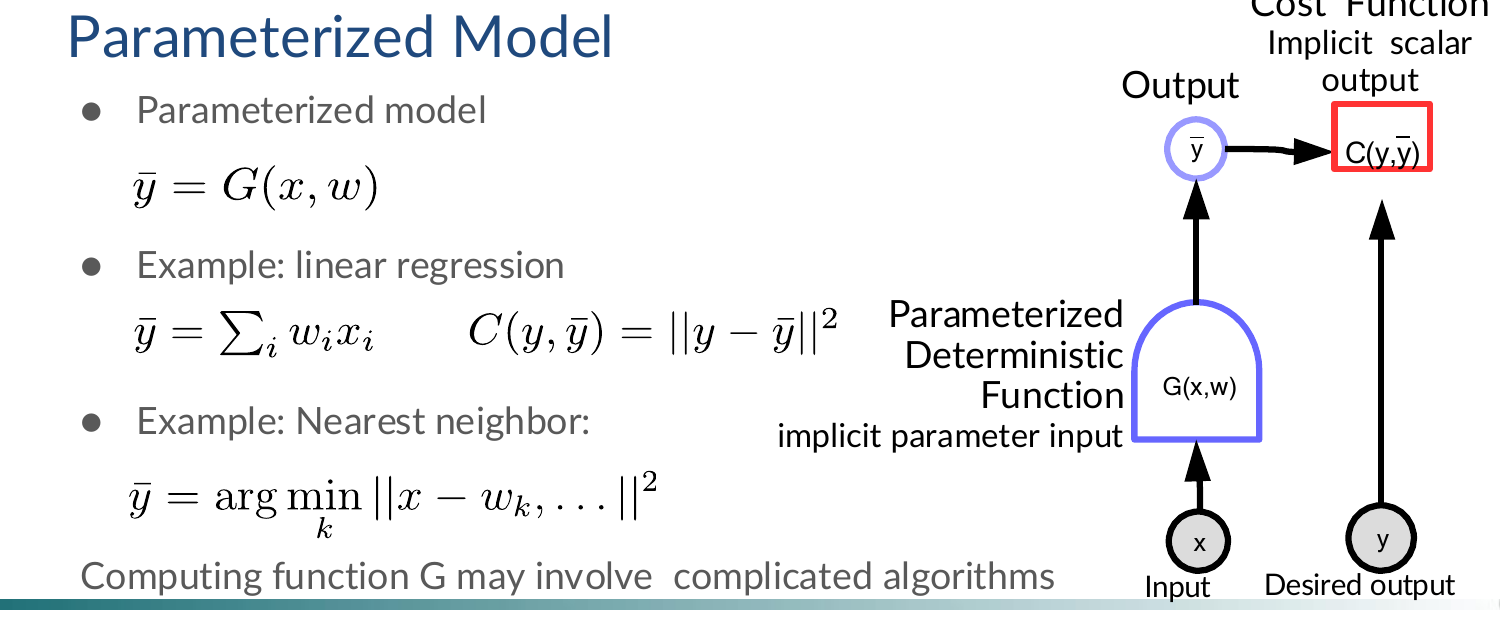
\includegraphics[width=0.88\linewidth]{figures/param_model.png}
  \caption{Schema del modello parametrico $\bar{y}=G(x,w)$. Il blocco
           $G(x,w)$ (rettangolo blu) prende in input $x$ e produce $\bar{y}$;
           la funzione di costo $C(y,\bar{y})$ (rettangolo rosso) ha output
           scalare implicito.}
  \label{fig:param_model}
\end{figure}

Due esempi fondamentali sono la \textbf{regressione lineare},
$\bar{y} = \sum_i w_i x_i$ con costo $C(y,\bar{y}) = \|y - \bar{y}\|^2$,
e il \textbf{k-Nearest Neighbor},
$\bar{y} = \arg\min_k \|x - w_{k,.}\|^2$,
dove i parametri $w_k$ coincidono con i prototipi del dataset di training.

\subsection{Notazione con grafi a blocchi}
\label{ssec:block-diagram}

Le slide del corso adottano una notazione grafica precisa per i grafi
computazionali \reflecun{W1}, illustrata nella figura seguente.

\begin{figure}[H]
  \centering
  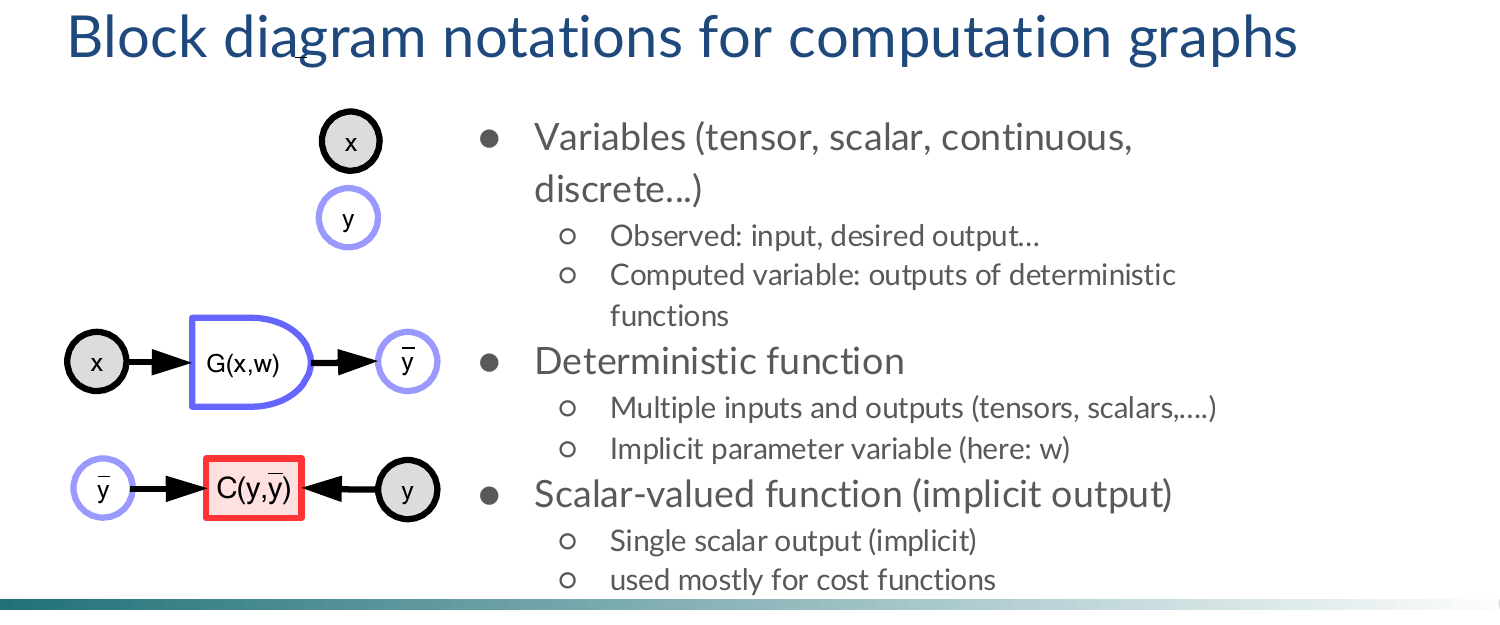
\includegraphics[width=0.82\linewidth]{figures/block_diagram.png}
  \caption{Notazione a blocchi per grafi computazionali: cerchi a bordo
           spesso = variabili osservate; cerchi a bordo sottile = variabili
           calcolate; rettangoli blu = funzioni deterministiche; rettangoli
           rossi = funzioni di costo con output scalare implicito.}
  \label{fig:block_diagram}
\end{figure}

\subsection{Funzione di loss e loss media}
\label{ssec:loss}

La \textbf{loss per campione} è $L(x, y, w) = C(y, G(x, w))$.
Dato il dataset $S = \{(x[p], y[p]) \mid p = 0, \ldots, P-1\}$,
la \textbf{loss media} è:
\begin{equation}
  \mathcal{L}(S,\, w)
  = \frac{1}{P}\sum_{p=0}^{P-1} L(x[p],\, y[p],\, w).
\end{equation}
L'obiettivo dell'apprendimento è $w^* = \arg\min_w \mathcal{L}(S,w)$.

\begin{figure}[H]
  \centering
  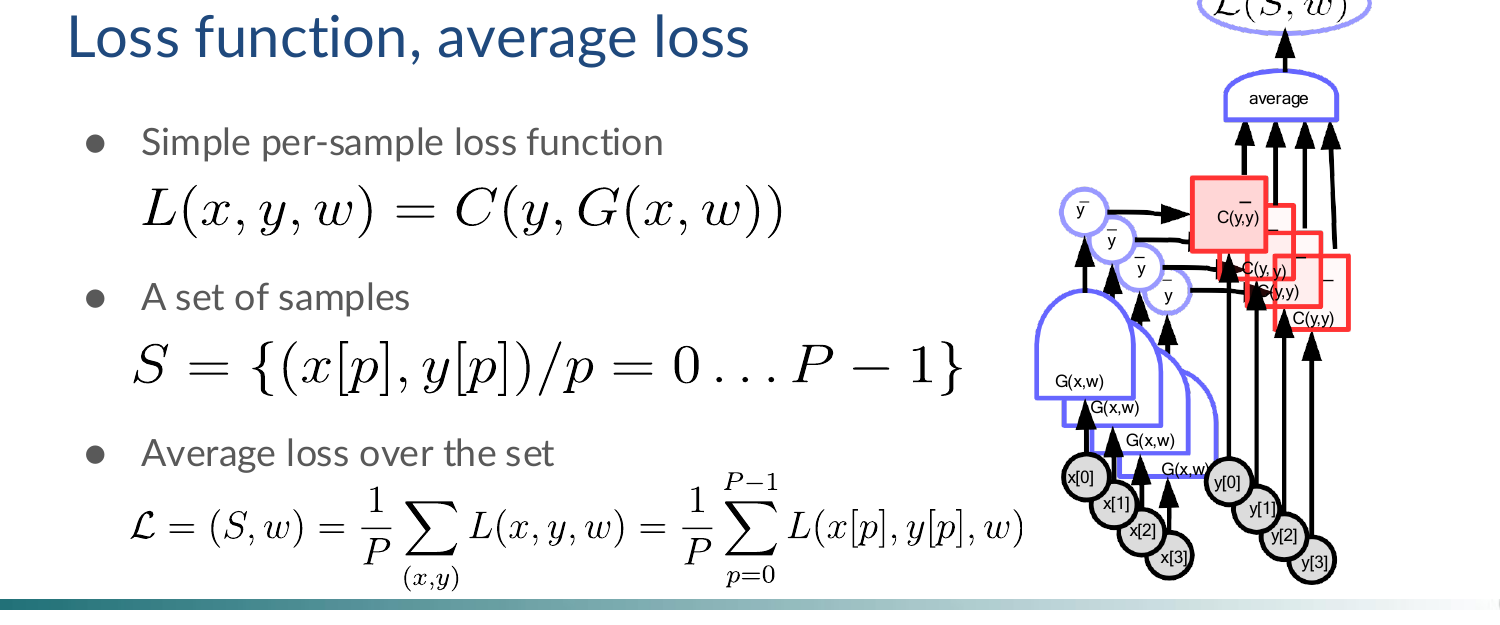
\includegraphics[width=0.88\linewidth]{figures/loss_avg.png}
  \caption{Grafo computazionale della loss media: il blocco $G(x,w)$ è
           replicato per ogni campione (con pesi condivisi) e le loss
           individuali $C(y,\bar{y})$ vengono mediate.}
  \label{fig:loss_avg}
\end{figure}

%------------------------------------------------------------
\section{Reti Neurali Tradizionali}
\label{sec:traditional-nn}

Una rete neurale tradizionale è una composizione alternata di blocchi
\textbf{lineari} e \textbf{non-lineari} \refbishop{6}:
\begin{align}
  s_{k+1} &= w_k\, z_k  \qquad &&\text{(blocco lineare)} \\
  z_k     &= h(s_k)             &&\text{(blocco non-lineare)}
\end{align}
dove $h(\cdot)$ è una funzione di attivazione punto per punto.
Per un neurone $i$, indicando con $UP(i)$ i neuroni del livello precedente:
\begin{equation}
  s[i] = \sum_{j \in UP(i)} w[i,j] \cdot z[j], \qquad z[i] = f(s[i]).
\end{equation}

\begin{figure}[H]
  \centering
  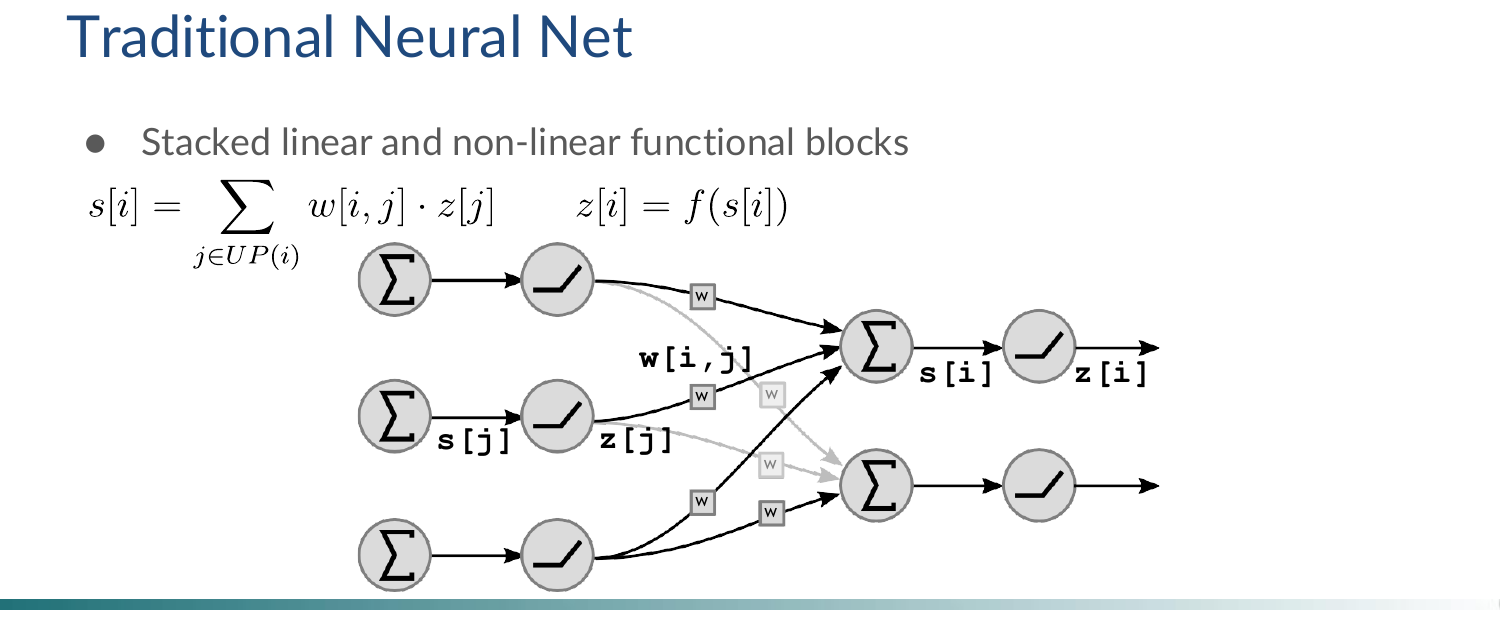
\includegraphics[width=0.88\linewidth]{figures/trad_nn.png}
  \caption{Struttura di una rete neurale tradizionale: i nodi $\Sigma$
           calcolano la somma pesata $s[i]$; i nodi con la curva applicano
           la non-linearità $z[i]=f(s[i])$; i riquadri $w$ rappresentano
           i pesi $w[i,j]$.}
  \label{fig:trad_nn}
\end{figure}

La catena lineare a blocchi per una rete a 3 layer è:
$x \xrightarrow{w_0} s_1 \xrightarrow{h} z_1 \xrightarrow{w_1} s_2
   \xrightarrow{h} z_2 \xrightarrow{w_2} s_3$.

\begin{figure}[H]
  \centering
  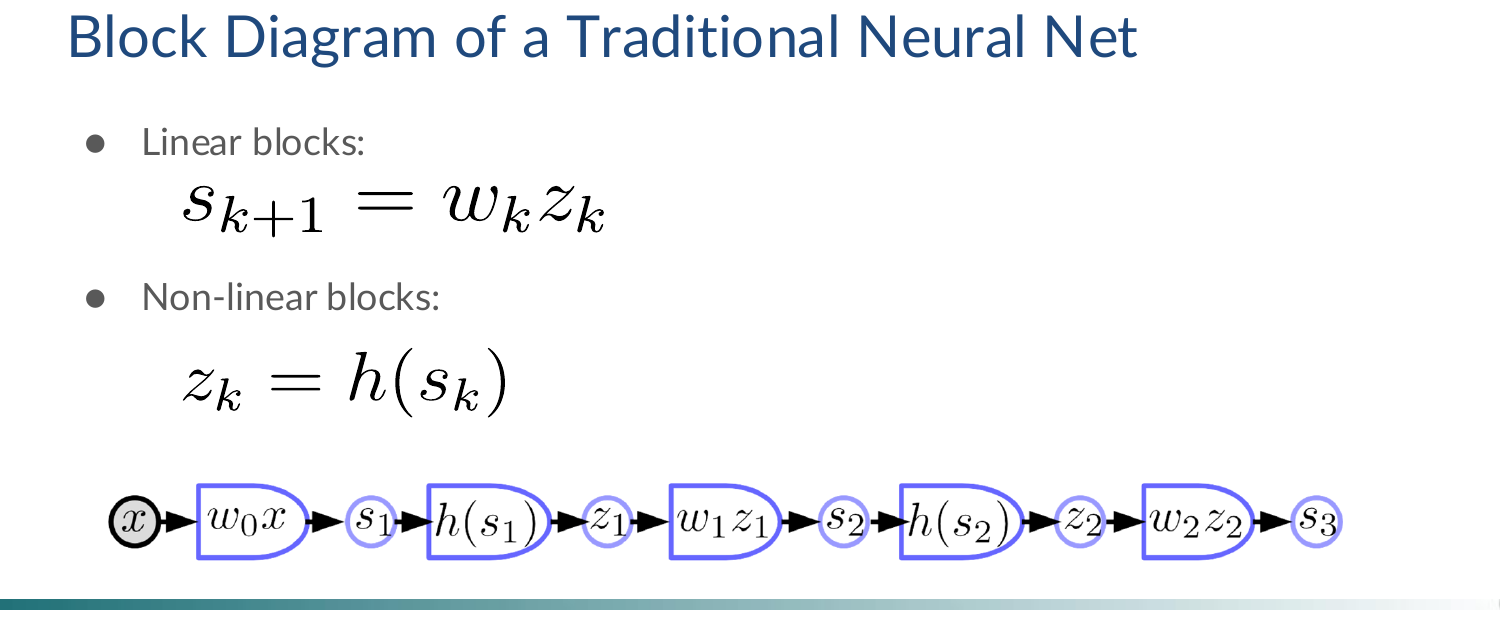
\includegraphics[width=0.88\linewidth]{figures/block_nn.png}
  \caption{Diagramma a blocchi di una rete a 3 layer: blocchi lineari
           (rettangoli) e non-lineari (forme arrotondate) si alternano.}
  \label{fig:block_nn}
\end{figure}

\subsection{Implementazione in PyTorch}

\begin{lstlisting}[language=Python, caption={MLP a 3 layer in PyTorch}]
import torch
from torch import nn

class MyNet(nn.Module):
    def __init__(self, d0, d1, d2, d3):
        super().__init__()
        self.m0 = nn.Linear(d0, d1)   # include bias
        self.m1 = nn.Linear(d1, d2)
        self.m2 = nn.Linear(d2, d3)

    def forward(self, x):
        z0 = x.view(-1)                # flatten
        z1 = torch.relu(self.m0(z0))
        z2 = torch.relu(self.m1(z1))
        return self.m2(z2)             # logit di output

model = MyNet(600, 60, 40, 10)
out   = model(torch.randn(3, 10, 20))
\end{lstlisting}

%------------------------------------------------------------
\section{Grafi Computazionali e Backpropagation}
\label{sec:backprop}

Un \textbf{grafo computazionale} è un DAG in cui i nodi foglia sono le variabili
di ingresso e i parametri, mentre i nodi interni rappresentano operazioni.
L'ordinamento topologico definisce l'ordine del forward e del backward pass
\refbishop{7}. Se il grafo contiene cicli (reti ricorrenti), è necessario
srotolarlo nel tempo (\textbf{BPTT}).

\subsection{Regola della catena -- caso scalare}

La backpropagation \citep{rumelhart1986} si fonda sulla \textbf{regola della
catena}: per $c = g(z)$, $z = h(s)$:
\begin{equation}
  \frac{dc}{ds} = \frac{dc}{dz} \cdot h'(s).
\end{equation}
Perturbando $s$ di $ds$ si perturba $z$ di $dz = h'(s)\,ds$, e quindi
$c$ di $dc = (dc/dz)\,dz$.

\begin{figure}[H]
  \centering
  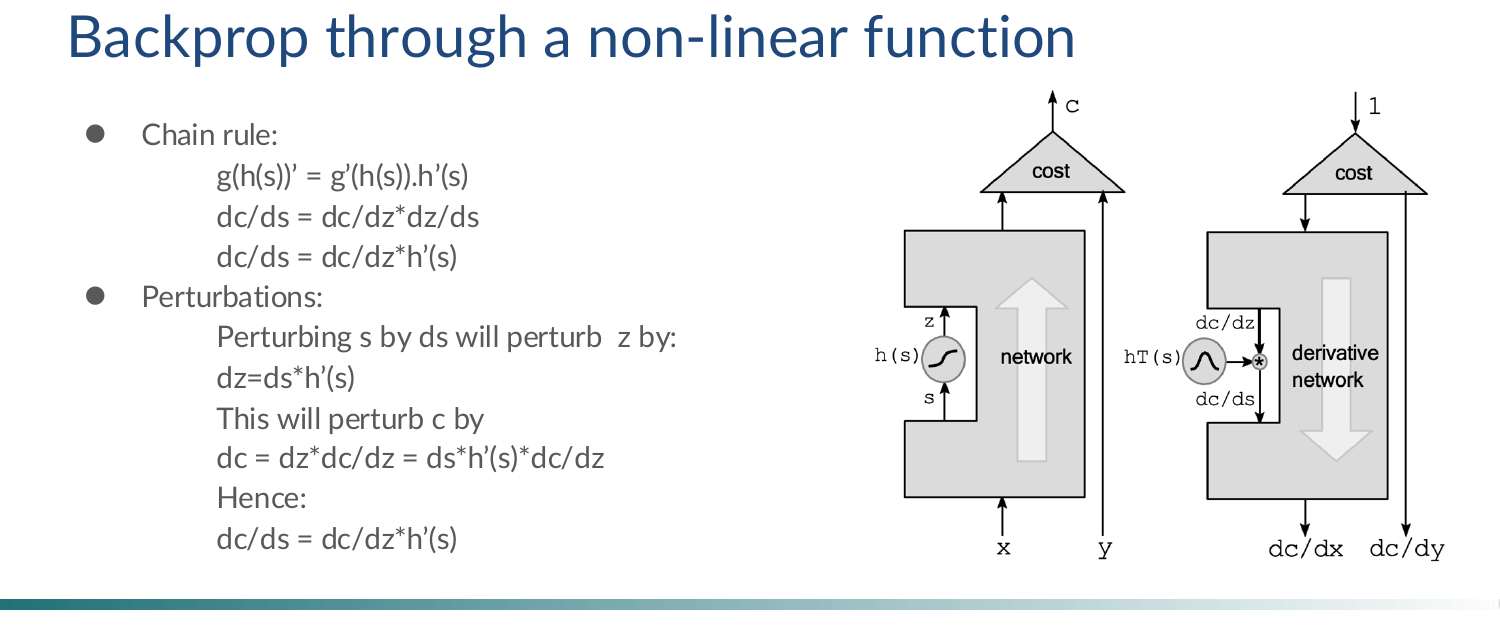
\includegraphics[width=0.82\linewidth]{figures/backprop_nonlin.png}
  \caption{Backprop attraverso una funzione non-lineare $h(s)$: la rete
           duale (destra) moltiplica il gradiente entrante $dc/dz$ per la
           derivata trasposta $h^T(s)$, producendo $dc/ds$.}
  \label{fig:backprop_nonlin}
\end{figure}

Per un neurone $z$ che alimenta più neuroni $s[0],s[1],s[2]$ tramite pesi
$w[0],w[1],w[2]$, il gradiente rispetto all'ingresso è la somma pesata:
\begin{equation}
  \frac{dc}{dz} = \sum_i \frac{dc}{ds[i]} \cdot w[i].
\end{equation}

\subsection{Caso vettoriale e matrice Jacobiana}

Per funzioni vettoriali con $z_f : [d_f \times 1]$ e $z_g : [d_g \times 1]$:
\begin{equation}
  \underbrace{\frac{\partial c}{\partial z_f}}_{[1 \times d_f]}
  = \underbrace{\frac{\partial c}{\partial z_g}}_{[1 \times d_g]}
    \cdot
    \underbrace{\frac{\partial z_g}{\partial z_f}}_{[d_g \times d_f]}.
\end{equation}
La \textbf{matrice Jacobiana} ha elemento $(i,j)$ uguale alla derivata
parziale della $i$-esima uscita rispetto alla $j$-esima entrata:
$(\partial z_g / \partial z_f)_{ij} = (\partial z_g)_i / (\partial z_f)_j$.

\begin{figure}[H]
  \centering
  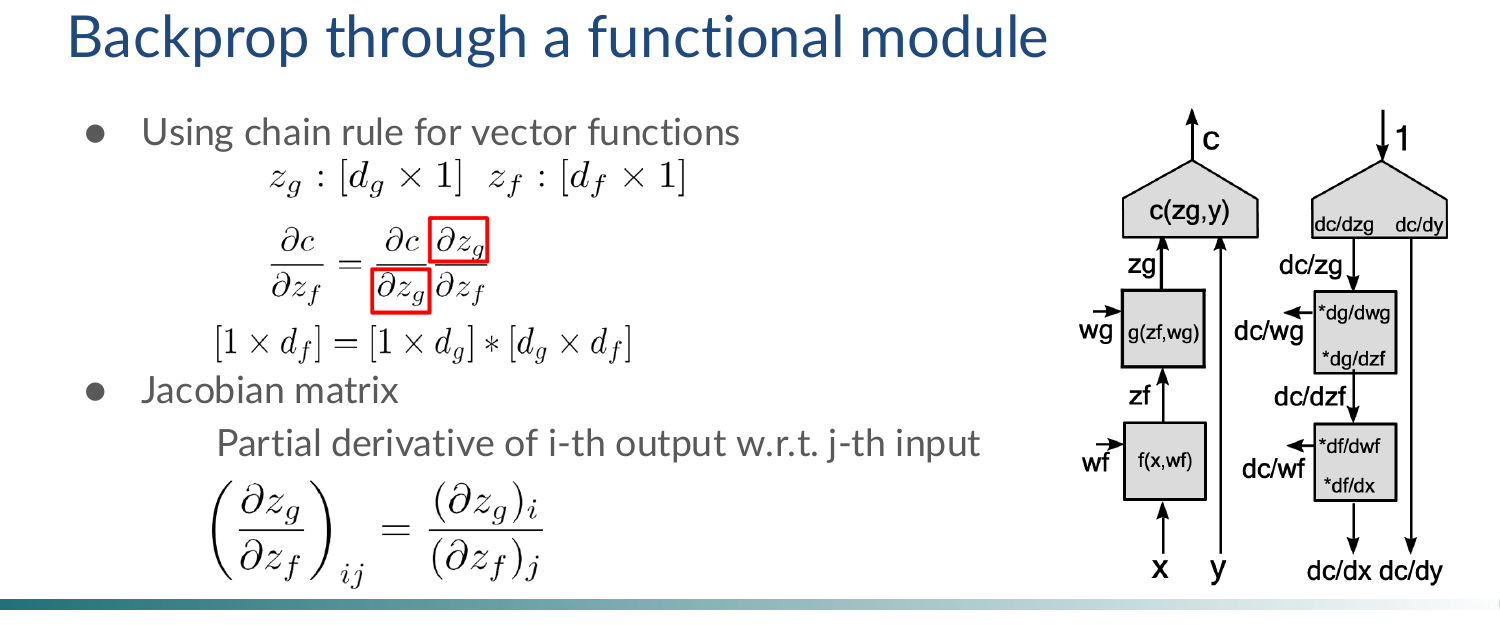
\includegraphics[width=0.88\linewidth]{figures/jacobian.png}
  \caption{Backprop attraverso un modulo vettoriale: ogni modulo espone
           due Jacobiane, una per i pesi ($*dg/dwg$) e una per l'ingresso
           ($*dg/dzf$), corrispondenti alle due frecce della rete duale.}
  \label{fig:jacobian}
\end{figure}

\subsection{Backprop in un grafo multi-stadio}

Per una rete a $K$ stadi con $z_{k+1} = f_k(z_k, w_k)$:
\begin{align}
  \frac{\partial c}{\partial z_k}
  &= \frac{\partial c}{\partial z_{k+1}}
     \cdot \frac{\partial f_k(z_k, w_k)}{\partial z_k}
  & &\text{(gradiente di stato)} \\
  \frac{\partial c}{\partial w_k}
  &= \frac{\partial c}{\partial z_{k+1}}
     \cdot \frac{\partial f_k(z_k, w_k)}{\partial w_k}
  & &\text{(gradiente dei pesi)}
\end{align}

\begin{figure}[H]
  \centering
  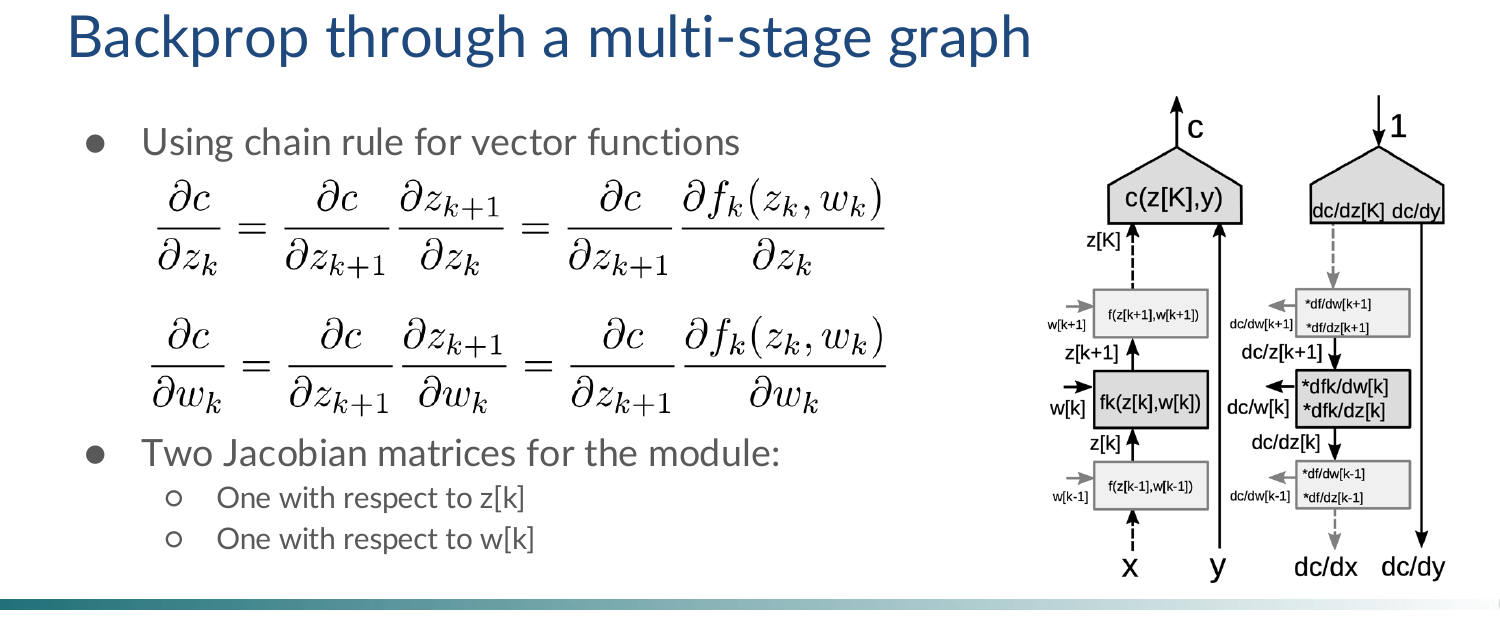
\includegraphics[width=0.88\linewidth]{figures/multistage.png}
  \caption{Backprop in un grafo multi-stadio: la rete duale (destra) esegue
           il forward pass ``al contrario'', con ogni modulo che produce due
           Jacobiane ($*dfk/dw[k]$ e $*dfk/dz[k]$).}
  \label{fig:multistage}
\end{figure}

La backpropagation è quindi una \textit{propagazione sul grafo duale}: ogni
nodo è sostituito dal suo modulo derivata, e il gradiente scende dall'output
verso l'input. Con $y,\bar{y}: [M\times1]$ e $w: [N\times1]$:
\begin{equation}
  \underbrace{\pd{C}{w}}_{[1\times N]}
  = \underbrace{\pd{C}{\bar{y}}}_{[1\times M]}
    \cdot
    \underbrace{\pd{\bar{y}}{w}}_{[M\times N]}.
\end{equation}

\begin{figure}[H]
  \centering
  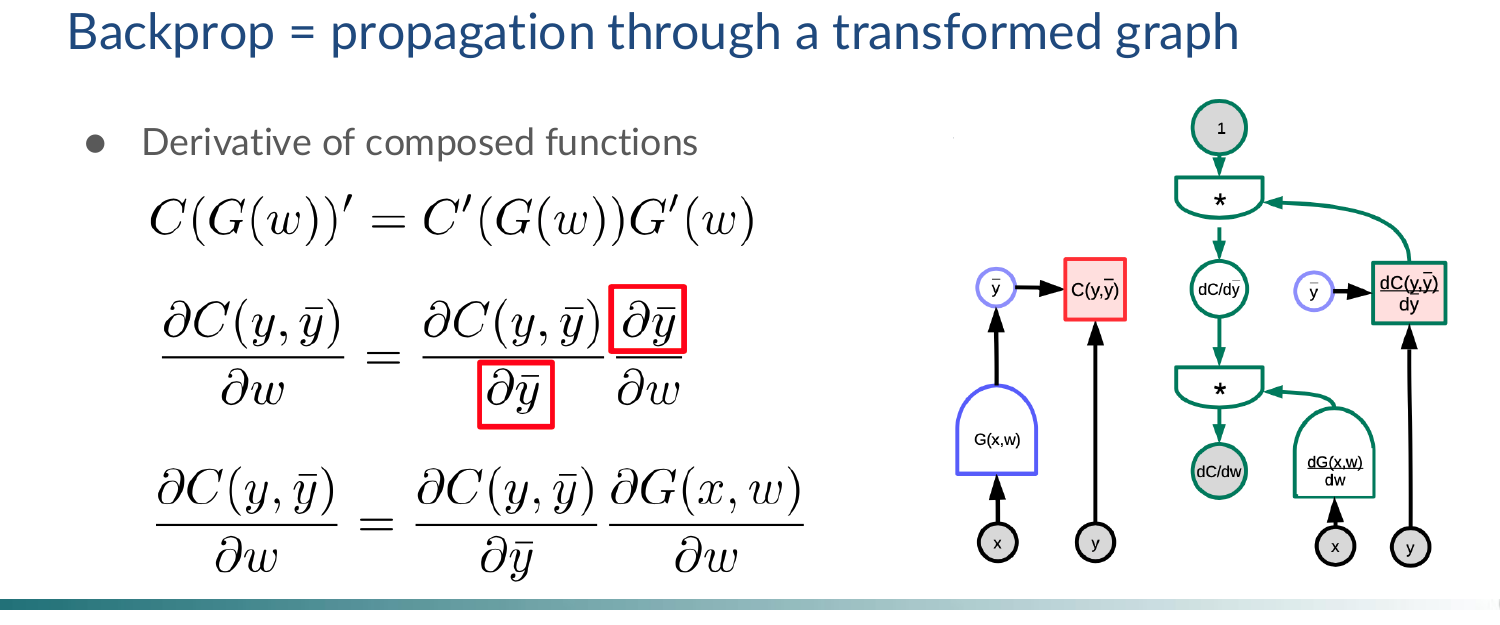
\includegraphics[width=0.82\linewidth]{figures/backprop_graph.png}
  \caption{Backprop come propagazione sul grafo duale: $\partial C/\partial w
           = (\partial C/\partial\bar{y})\cdot(\partial G/\partial w)$.}
  \label{fig:backprop_graph}
\end{figure}

La backpropagation è applicabile a qualsiasi DAG. Se il grafo ha cicli
(reti ricorrenti) occorre srotolarlo nel tempo (BPTT).

\begin{figure}[H]
  \centering
  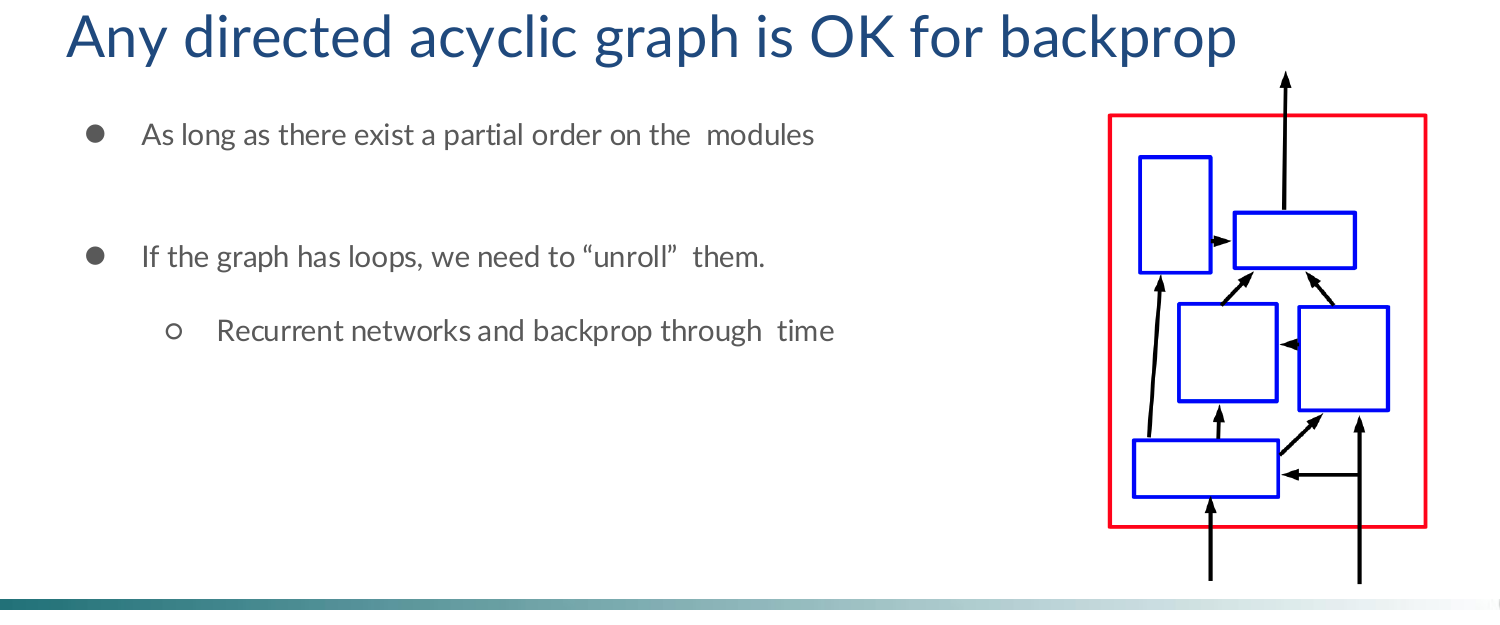
\includegraphics[width=0.55\linewidth]{figures/dag_backprop.png}
  \caption{Un esempio di DAG con flusso di dati in avanti (frecce nere) e
           backprop (frecce rosse) che lo percorre in senso inverso.}
  \label{fig:dag_backprop}
\end{figure}

%------------------------------------------------------------
\section{Riepilogo}
\label{sec:summary-ch0}

\begin{center}
\begin{tabular}{lll}
  \toprule
  \textbf{Concetto} & \textbf{Formula} & \textbf{Ruolo} \\
  \midrule
  Modello param.  & $\bar{y}=G(x,w)$                  & Base di ogni sistema ML \\
  Loss media      & $\mathcal{L}=\frac{1}{P}\sum_p C$  & Obiettivo \\
  Blocco lineare  & $s_{k+1}=w_k z_k$                  & Trasformazione affine \\
  Blocco non-lin. & $z_k=h(s_k)$                       & Capacità non-lineare \\
  Chain rule      & $dc/ds=(dc/dz)h'(s)$               & Motore backprop \\
  Jacobiano       & $(\partial z_g/\partial z_f)_{ij}$  & General.\ vettoriale \\
  DAG + backprop  & $\partial c/\partial z_k = \partial c/\partial z_{k+1}\cdot\partial f_k/\partial z_k$ & Algoritmo generale \\
  \bottomrule
\end{tabular}
\end{center}
